
%(BEGIN_QUESTION)
% Copyright 2014, Tony R. Kuphaldt, released under the Creative Commons Attribution License (v 1.0)
% This means you may do almost anything with this work of mine, so long as you give me proper credit

Determine the input frequency necessary to give the output voltage a phase shift of 40$^{o}$:

$$\includegraphics[width=15.5cm]{i01063x01.eps}$$

\underbar{file i01063}
%(END_QUESTION)





%(BEGIN_ANSWER)

$f$ = 6.54 kHz

%(END_ANSWER)





%(BEGIN_NOTES)

Phase-shifting circuits are very useful, and important to understand.  They are particularly important in some types of oscillator circuits, which rely on RC networks such as this to provide certain phase shifts to sustain oscillation.

%INDEX% Electronics review: AC reactance and impedance

%(END_NOTES)


